\documentclass[a4paper, 11pt]{article}
	\usepackage[utf8]{inputenc}
    \usepackage[french]{babel}
    \usepackage[T1]{fontenc}
    \usepackage[top=3cm,, right=2cm,bottom=2cm,left=2cm]{geometry}
    \usepackage{eurosym} %pour le symbole euro

    \usepackage{tabularx}
    \usepackage{soul}
		\usepackage{enumitem}

		\usepackage{pdfpages}

    \title{Hackerspace Au Mans}
    \author{Procès-Verbal des Assemblées Générales Ordinaire et Extraordinaire}
    \date{Le jeudi 14 Juillet 2022}

    \newcommand\sep{\noindent\rule{\linewidth}{.5pt}}

    \newcommand{\vote}[5]{

    \smallskip
    \fbox{\begin{minipage}[l]{\textwidth}
    	\smallskip
        \begin{center}
        	\ul{\textsc{Vote}}
        \end{center}

        #1\\
        \textbf{Votants} #2\\
        \textbf{Pour} #3\\
        \textbf{Contre} #4\\
        \textbf{NSPP} #5

        \smallskip

    \end{minipage}}
        \medskip
    }

    \newcommand\question[2]{\noindent\ul{\textit{\textsc{$\bullet$ #1}}}\\#2\\}

    %\ul{#2}}


\begin{document}

\maketitle

\section{Effectifs}

\begin{itemize}
	\item Présents :
		\begin{itemize}
    		\item CONTY Romuald
    		\item FAVREAU Tifenn
			\item TOUCHARD Florent
			\item GABORIT Mathieu
			\item BRÉHÉRET Jérôme
			\item VANNIER Laurent
    		\item VALLÉE Sébastien
    		\item JORANT Baptiste (arrivée à 15h20)
		\end{itemize}
\end{itemize}

\bigskip

%%La présidence actuelle décide d'accorder le droit de vote à tous les présents pour la durée de cette AG.
\setlist{nosep,after=\vspace{\bigskipamount}}

\section{Assemblée générale ordinaire}
\textbf{La séance est ouverte à 15h00}
\subsection*{Préambule}

Le président donne droit de vote à l'ensemble des personnes majeures présentes.

\subsection{Rapport Moral}

Le rapport moral (cf annexe) est présenté par le président.

Début du vote à 15h15.

\vote{Rapport moral}{7}{7}{0}{0}

Le rapport moral est validé par l'assemblée.

\subsection{Rapport Financier}

La trésorière présente le rapport financier (cf annexe).

Début du vote à 15h27.

\vote{Rapport financier}{8}{8}{0}{0}

Le rapport financier est validé par l'assemblée.

\subsubsection{Question et remarques sur le rapport financier}

La trésorière demande si la prestation Le Mans Sonore (2022) a bien été facturée, 
car, à ce jour, aucun paiement n'a été recu pour cette prestation. 

Réponse : Jérome doit envoyer un mail pour relancer Teriaki sur le paiement de cette
prestation, la facturation étant déja faite.

%====================================================================================

\subsection{Motions}

\subsubsection{Modification des conditions d'adhésions des membres partenaires : Article 2 du réglement intérieur}

La motion est présentée par le président.

Début du vote à 15h33.

\vote{Motion sur la modification des conditions d'adhésion des membres partenaires}{8}{8}{0}{0}

La motion est validée par l'assemblée.

\subsubsection{Suppression de la facturation spécifique pour l'usage du materiel : Article 9 du réglement intérieur}

La motion est présentée par le président.

Début du vote à 15h35.

\vote{Motion sur l'adhésion des membres partenaires}{8}{8}{0}{0}

La motion est validée par l'assemblée.

\subsection{Élection du bureau}

Se présentent à l'élection au bureau :

\begin{itemize}
	\item BREHERET Jérôme
	\item CONTY Romuald
	\item GABORIT Mathieu
	\item TOUCHARD Florent
	\item VALLÉE Sébastien
	\item VANNIER Laurent
\end{itemize}
Début du vote à 15h39
\\
   \hspace{-1cm} \fbox{\begin{minipage}{1.06\textwidth}
    		\smallskip
       		\begin{center}
        		\ul{\textsc{Vote}}\\
        		Élection au bureau de
      	 	\end{center}

       		\begin{tabularx}{2\textwidth}{p{2.6cm} | p{2.6cm} | p{2.6cm} | p{2.6cm} | p{2.6cm} | p{2.6cm} }
						\small \textsc{BRÉHÉRET} \mbox{Jérôme} &
						\small \textsc{CONTY} \mbox{Romuald} &
						\small \textsc{GABORIT} \mbox{Mathieu} &
						\small \textsc{TOUCHARD} \mbox{Florent} &
						\small \textsc{VALLÉE} \mbox{Sébastien} &
						\small \textsc{VANNIER} \mbox{Laurent}
						\\
						\small \textbf{Votants} 8 &
						\small \textbf{Votants} 8 &
						\small \textbf{Votants} 8 &
						\small \textbf{Votants} 8 &
						\small \textbf{Votants} 8 &
						\small \textbf{Votants} 8
						\\
       		 			\textbf{Pour} 8 &
						\textbf{Pour} 8 &
						\textbf{Pour} 8 &
						\textbf{Pour} 8 &
						\textbf{Pour} 8 &
						\textbf{Pour} 8
						\\
        		\textbf{Contre} 0 &
						\textbf{Contre} 0 &
						\textbf{Contre} 0 &
						\textbf{Contre} 0 &
						\textbf{Contre} 0 &
						\textbf{Contre} 0
						\\
						\textbf{NSPP} 0 &
						\textbf{NSPP} 0 &
						\textbf{NSPP} 0 &
						\textbf{NSPP} 0 &
						\textbf{NSPP} 0 &
						\textbf{NSPP} 0
						\\
            \smallskip
    		\end{tabularx}
    \end{minipage}}
        

		         \medskip

\textbf{La séance est levée à 15h40}

\section{Assemblée générale extraordinaire}
\textbf{La séance est ouverte à 15h40}
\subsection*{Préambule}

Cette assemblée générale extraordinaire a pour but de modifier le siège social ainsi 
que la modification de l'article 9 des statuts de l'association concernant les conditions
d'organisation des différentes assemblées régissant l'association.

\subsection{Modification du siège social : Article 3 des statuts}

Le président présente la motion consistant à modifier le siège social de l'association 
pour refléter le lieu d'occupation de celle ci.

Début du vote à 15h42

\vote{Modification du siège social de l'association}{8}{8}{0}{0}

La modification est validée par l'assemblée.

\subsection{Modification des conditions d'organisations des assemblées : Article 9 des statuts}

Le président présente la motion consistant à modifier cet article des statuts pour 
modifier les conditions d'organisation des différentes assemblées, et rendre ces 
conditions plus souples.

Début du vote à 15h44

\vote{Modification des conditions d'organisations des assemblées}{8}{8}{0}{0}

La modification est validée par l'assemblée.

\textbf{La séance est levée à 15h45}

\section{Réunion de bureau}

Alors que l'ensemble des membres du nouveau bureau est présent, il est décidé de procéder dans l'immédiat aux élections internes à celui-ci. Pour les votes suivants, le collège électoral est réduit au bureau seul (soient 6 membres).

Début du vote à 15h57
\vote{Jérôme BRÉHERET au poste de président}{6}{6}{0}{0}
\vote{Mathieu GABORIT au poste de trésorier}{6}{6}{0}{0}
\vote{Florent TOUCHARD au poste de vice-trésorier}{6}{6}{0}{0}
\vote{Sébastien VALLÉE au poste de secrétaire}{6}{6}{0}{0}
\vote{Laurent VANNIER au poste de vice-secrétaire}{6}{6}{0}{0}


\section{Composition du bureau}
\begin{description}
  \item[Président] Jérôme BRÉHÉRET
  \item[Trésorier] Mathieu GABORIT
  \item[Vice-Trésorier] Florent TOUCHARD
  \item[Secrétaire] Sébastien VALLÉE
  \item[Vice-Secrétaire] Laurent VANNIER
  \item[Membre du bureau] Romuald CONTY
\end{description}

La composition du bureau est validé par l'assemblée.
\bigskip

\textbf{La séance est levée à 16h00.}

\bigskip\bigskip

\sep

\bigskip\bigskip

Le présent procès-verbal est approuvé par le président du HAUM.

\bigskip\bigskip

Président :



\newpage

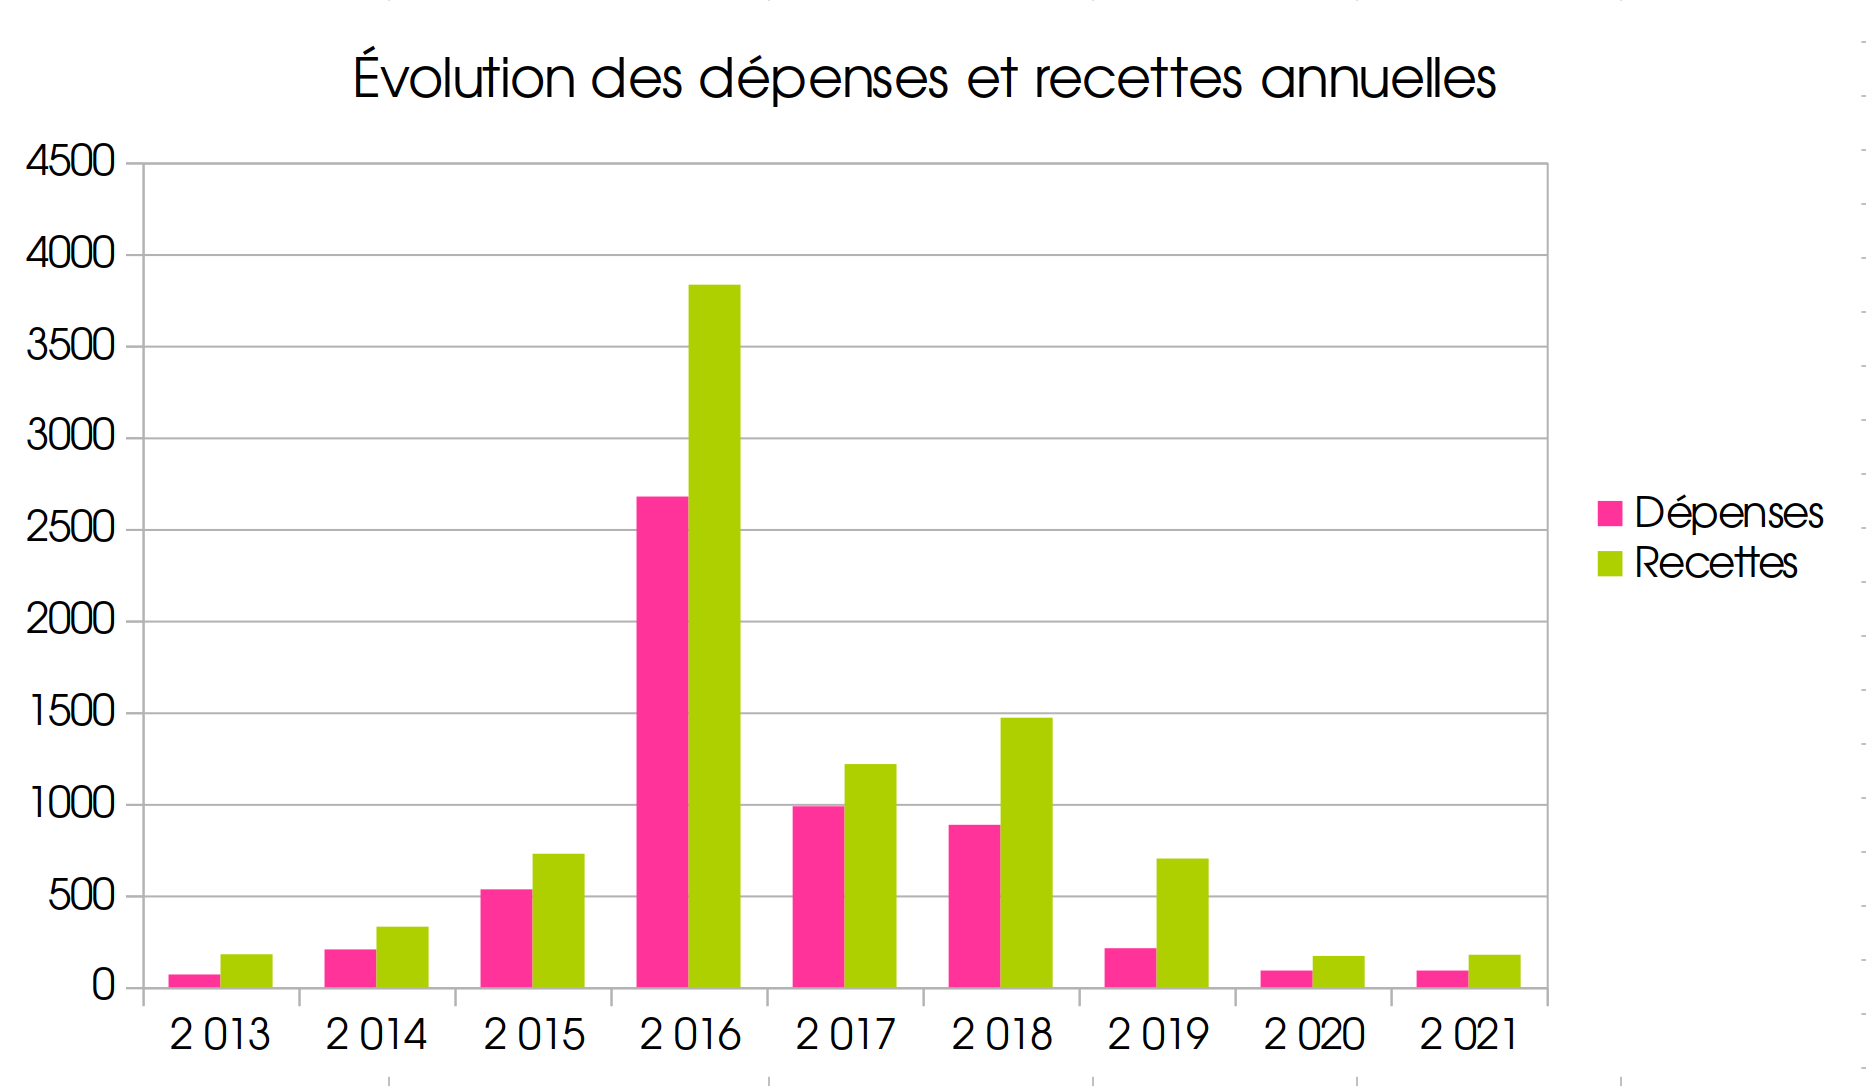
\includepdf[pages=-]{../convocation/3DossierAGGeneral2021.png}
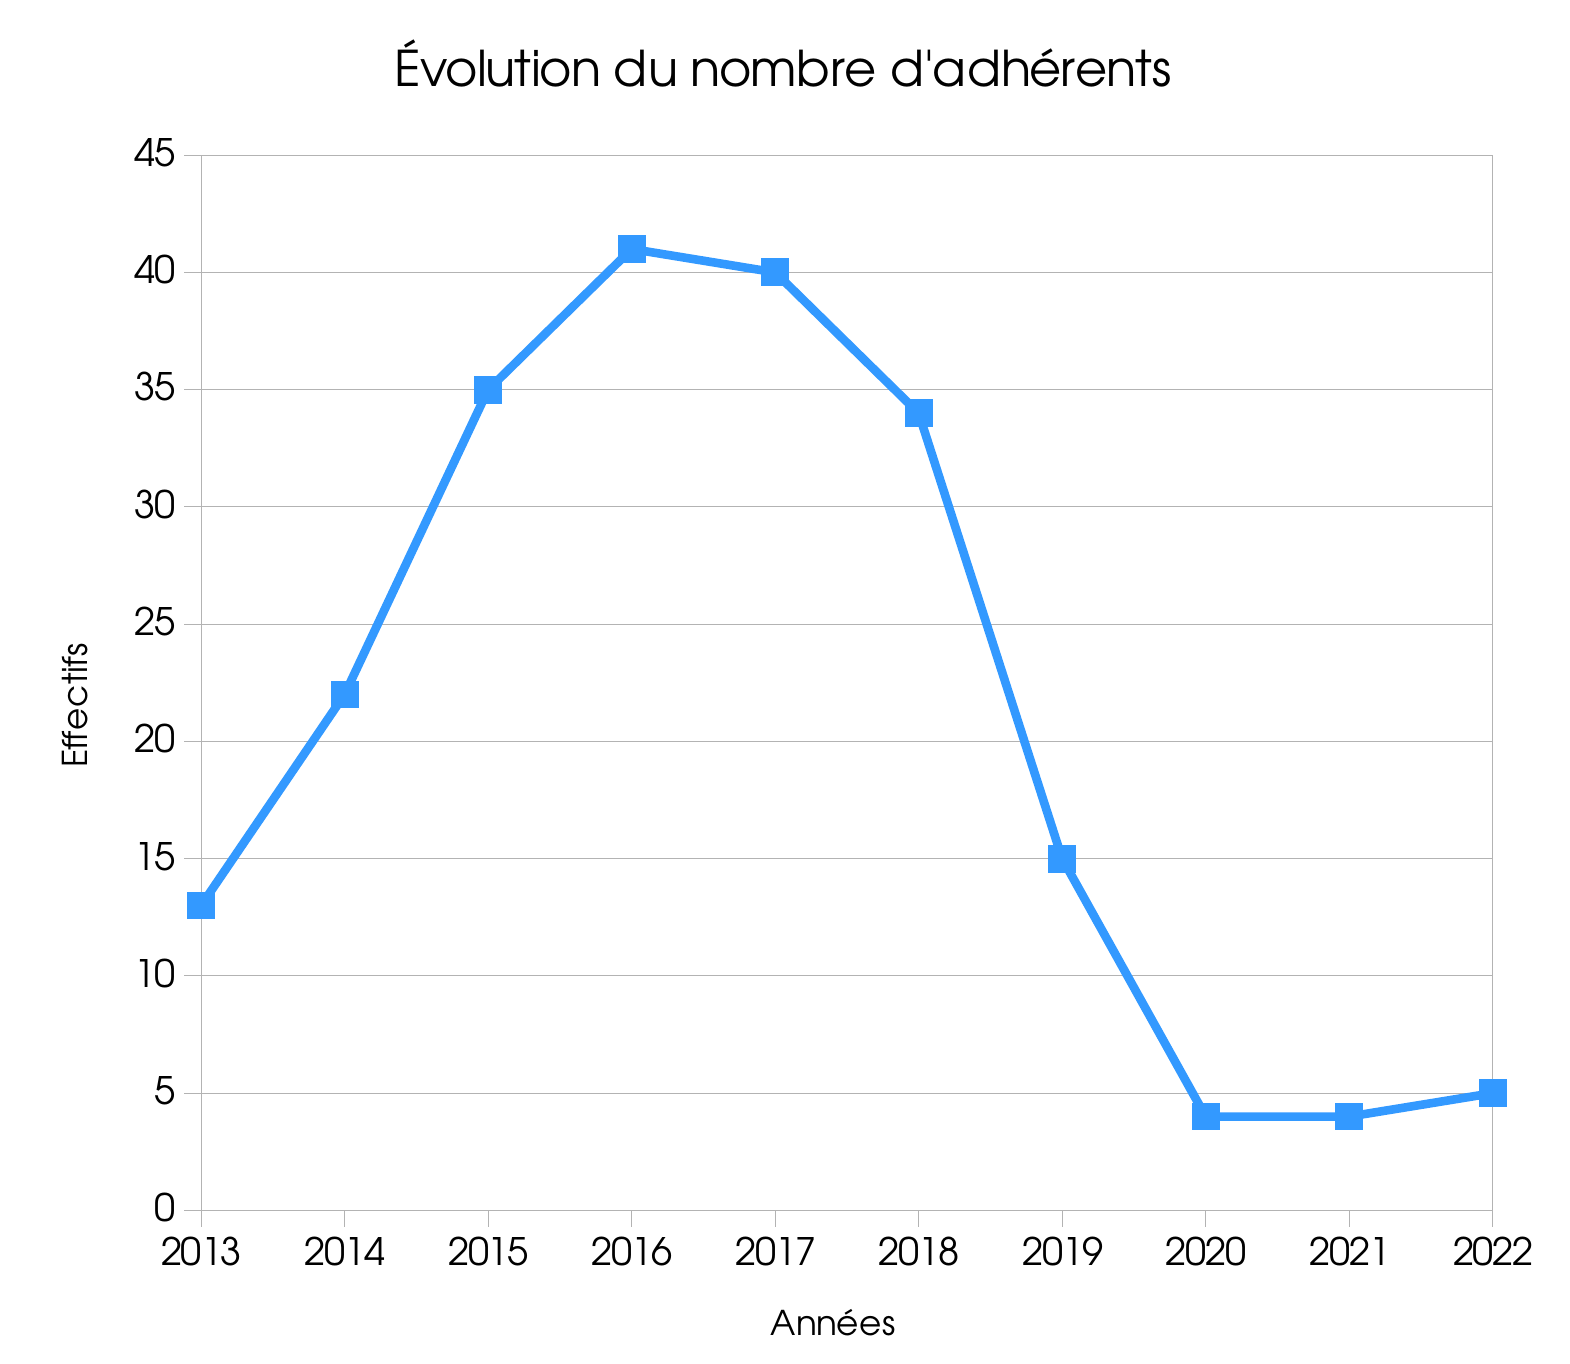
\includepdf[pages=-]{../convocation/4DossierAGAdherents2021.png}
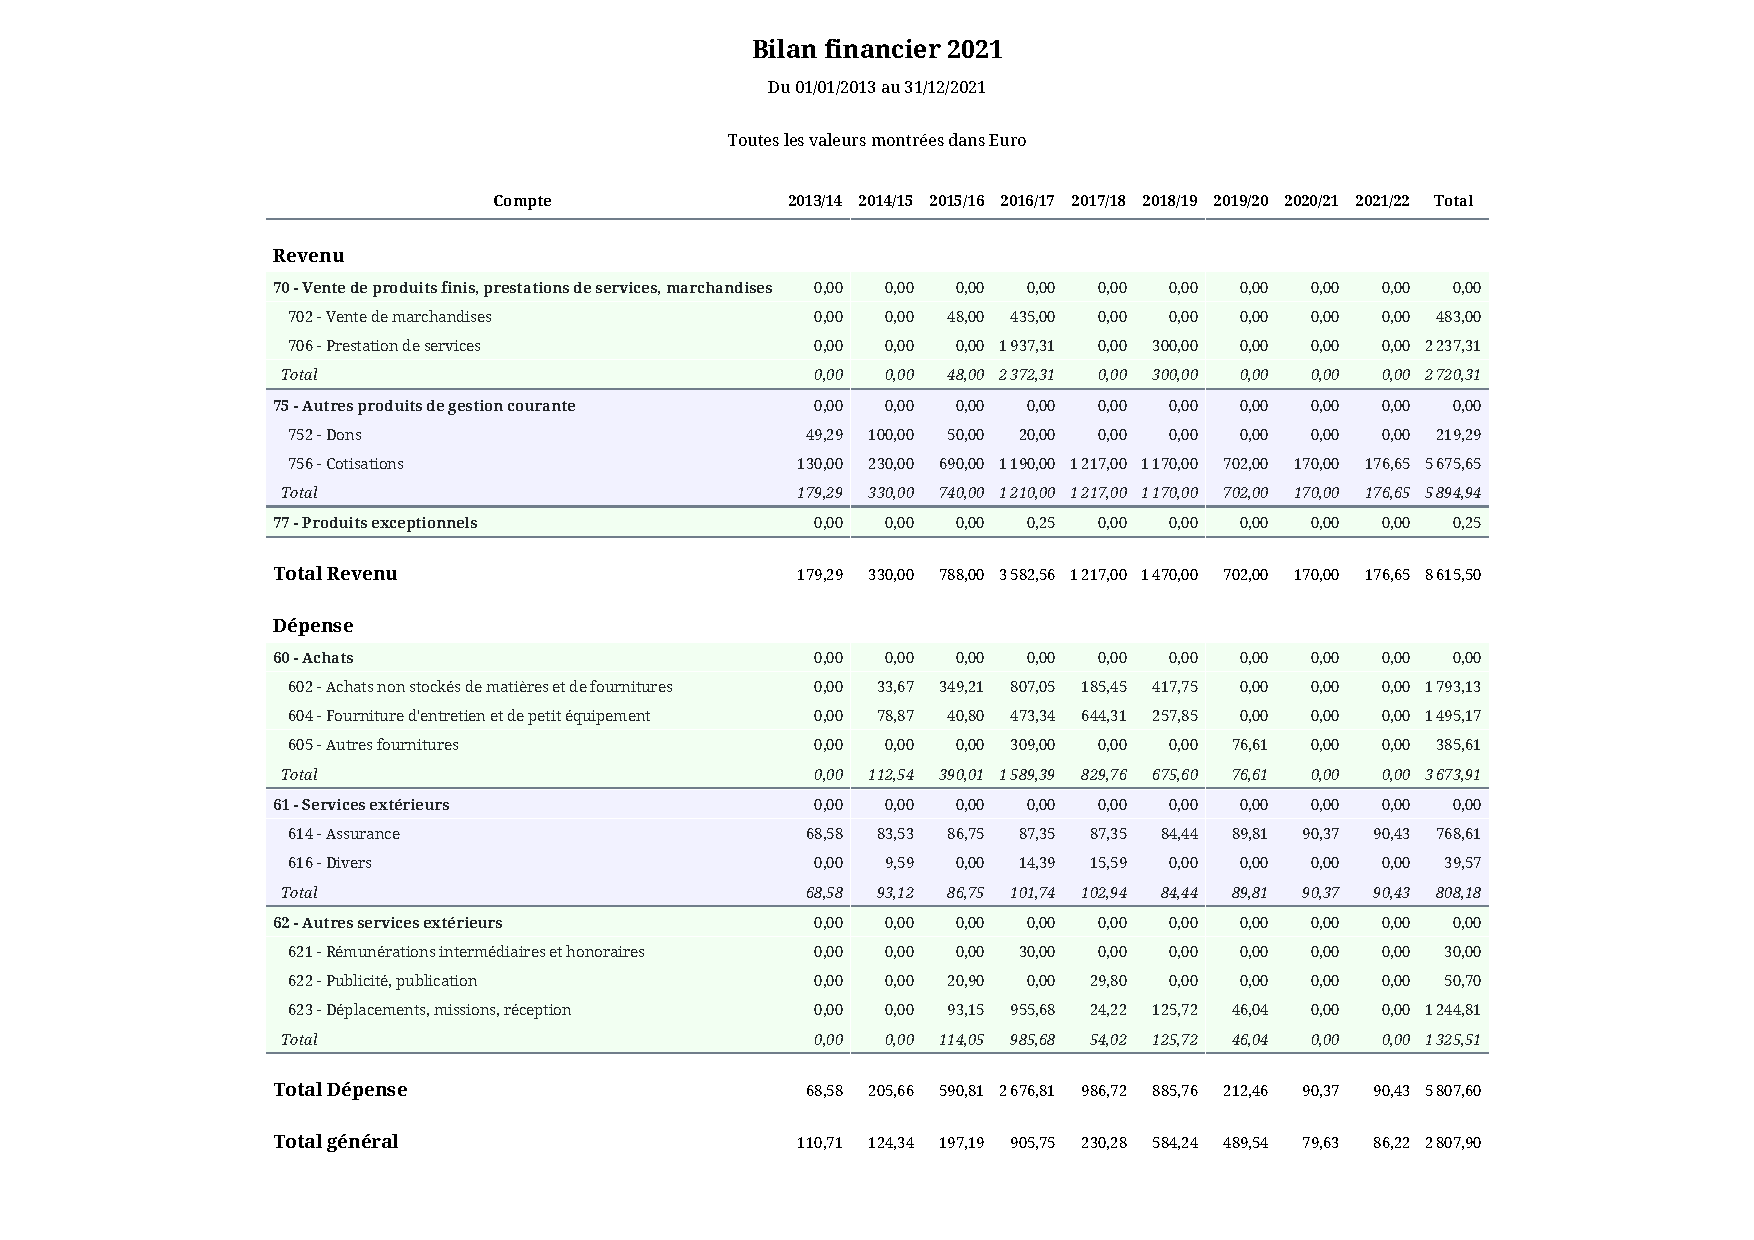
\includepdf[pages=-]{../convocation/BilanGénéral2021.pdf}
